\section{Motivation}\label{1_1_motivation}
%- Interactive real time feedback system in other sports
With the release of the Microsoft Kinect in 2010 a new area of game interaction has been released.
Already existing interaction devices like the Nintento Wii or PlayStation Move provide a remote control with motions sensors as the controlling device.
However, the Microsoft Kinect followed another approach by tracking the entire body of the user with an infrared sensor.
This resulted in various interaction possibilities, since no controlling device is needed and the full body could be tracked.
Especially fitness applications with exercises in which the user is in need of both hands or should not be disturbed by any other device benefited from this (see Figure~\ref{fig:1_kinectSports}).
\begin{figure}[htb]
	\centering
	\begin{minipage}[t]{1\linewidth}
		\centering
		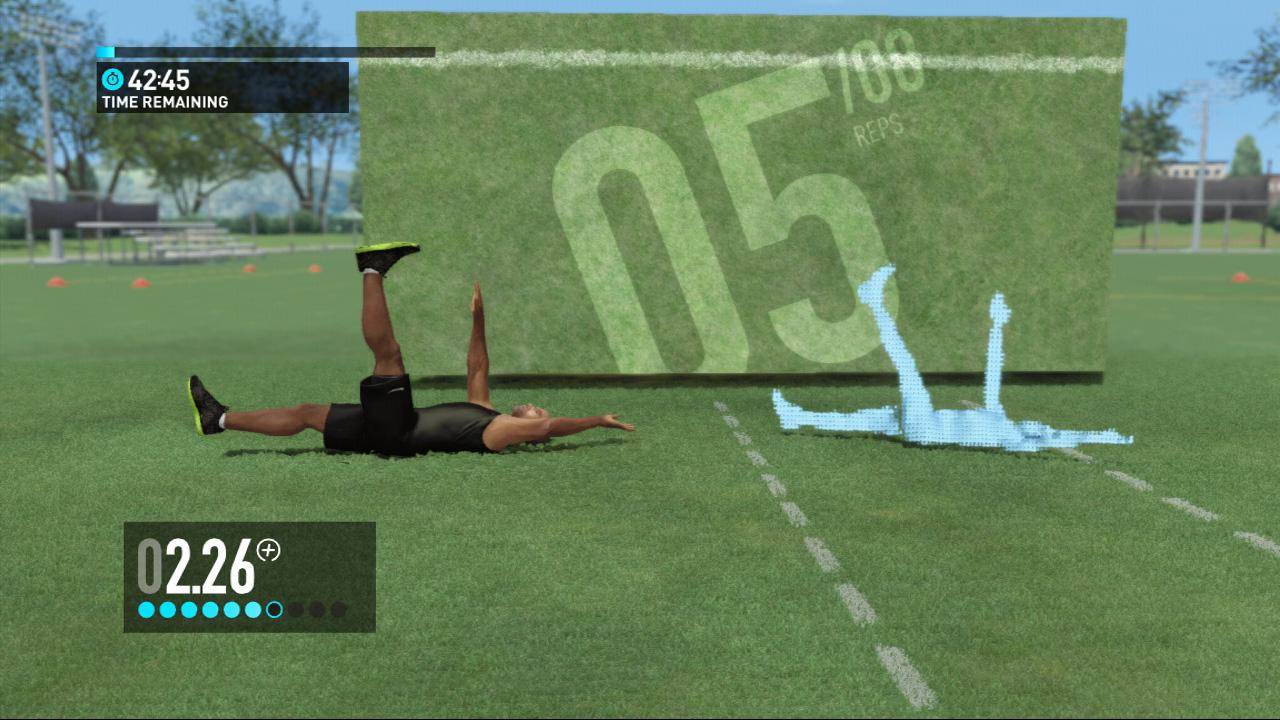
\includegraphics[width=0.55\linewidth]{Pictures/1_nikePlusKinect2}
		\caption{Ingame screenshot of the \textit{Nike+ Kinect Training}\protect\footnotemark Application. A virtual avatar demonstrates the exercise on the left side. The user can see herself mirorred on the right side of the screen.}
		\label{fig:1_kinectSports}
	\end{minipage}
\end{figure}
\footnotetext{\url{https://marketplace.xbox.com/de-DE/Product/Nike-Kinect-Training/66acd000-77fe-1000-9115-d8024d53090f}}

\begin{comment}
With the release of the Nintendo Wii in year 2006 a new area of game interaction has been released.
Whereas in common gaming console the main interaction was provided via buttons and analog sticks the Wii provided a remote controller with motion sensors. 
The position and movement of the user can be hereby located and adapted in the actual application.
This offered new possibilities of interaction in which motion based gaming application found its place.

For example in a baseball game the controller represents the hands of the virtual avatar (Figure~\ref{fig:1_wiiSportsTennis}).
The user swings the controller like in the real world to throw a ball.
In this way specific characteristics of games were more realistic, since the motions of the controller could be adapted to actions in the virtual gaming application.
\begin{figure}[htb]
	\centering
	\begin{minipage}[t]{1\linewidth}
		\centering
		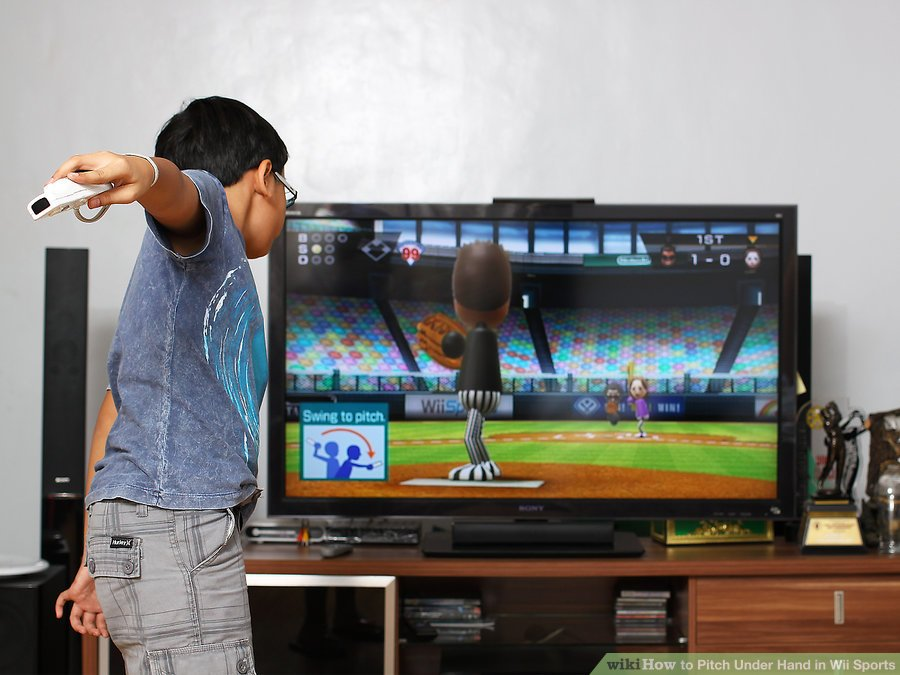
\includegraphics[width=0.55\linewidth]{Pictures/1_wiiSportTennis}
		\caption{asdasd}
		\label{fig:1_wiiSportsTennis}
	\end{minipage}
\end{figure}

Other manufacturers conquered with their own systems.
The PlayStation Move implemented a similar approach like the Nintendo Wii, with a remote controller.
However, the interaction of these devices are still restricted to a controller.
The Microsoft Kinect followed another approach by tracking the entire body of the user and building a skeleton.
It was possible to interact without any controlling device but just with the users‘ hands.
This again resulted in even more interaction possibilities, since the full body could be tracked.
Especially fitness application with exercises in which the user needs both hands or should not be disturbed by any other device, like push ups or crunches (Figure~\ref{fig:1_kinectSports}).

\begin{figure}[htb]
	\centering
	\begin{minipage}[t]{1\linewidth}
		\centering
		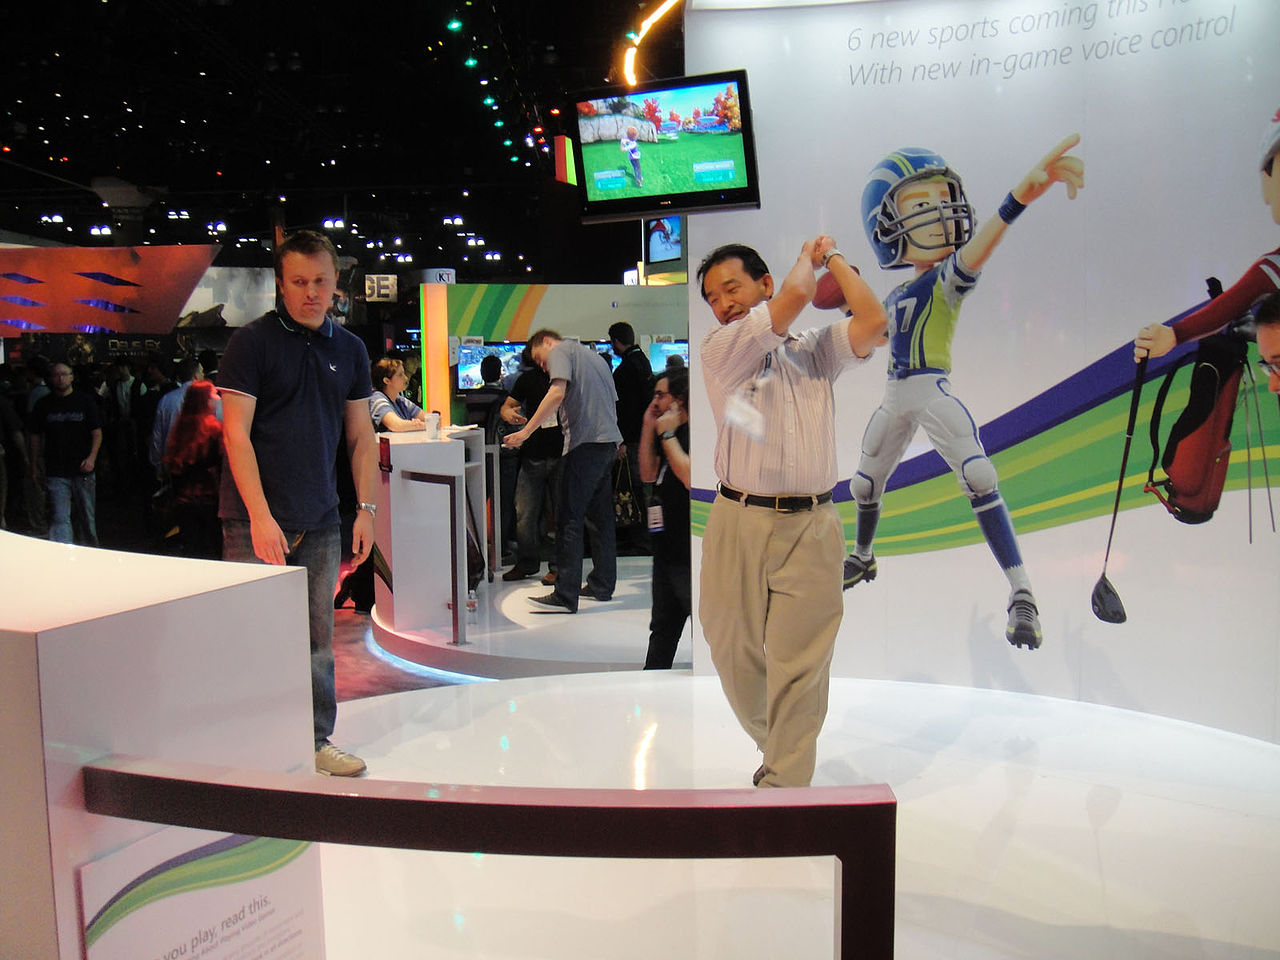
\includegraphics[width=0.55\linewidth]{Pictures/1_kinectSports}
		\caption{A user swinging his hands to control a virtual golf bat in Kinect Sports~\cite{Wiki2017-ksport}}
		\label{fig:1_kinectSports}
	\end{minipage}
\end{figure}
\end{comment}

Combining exercises that are implemented in a video game or a gamified environment and tracking the body movement of the user with an appropriate device originated in a new genre named \textit{exergames}~\cite{Buddharaju2016-ex, Sinclair2007-ex}.
Nowadays the uprising modern sedentary way of life , through more and more sitting jobs or watching television at home, leads to insufficient movement throughout the day.
Exergames can bring more contrast into their daily routine if implemented effectively~\cite{Rudella2012-ex}.
Several studies point out that such applications can improve the physical activity level, increase the engagement of the user, promote exercises, and provide an enjoyable experience~\cite{Graf2009-ex, Hicks2010-ex, Thin2010-ex}.
Further works have also shown that interactive system applications with an exergame approach can improve and train sport specific skill acquisition, e.g. in trampoline or climbing ~\cite{Bogdanovych2015-ci, Medeiros2017-ex, Holsti2013-kn, Jensen2014-ex, Kajastila2016-ot}.

Slacklining is a more specific form of sport that relies on the balance of the user.
She has to walk over a narrow ribbon, which is in general tensed between two static end points and about the height of 50 cm.
The length of the line varies from 3 up to 100 meters and more.
In general a beginner learns to balance on a slackline on her own with repetitive trials.
This can be frustrating and dangerous because she has to learn it by herself without any knowledge about the correct movements and body position.
Another approach is to learn it under experienced guidance with a well known expert.
However, the trainee must know such a person and is also dependent on her.
\begin{figure}[htb]
	\centering
	\begin{minipage}[t]{1\linewidth}
		\centering
		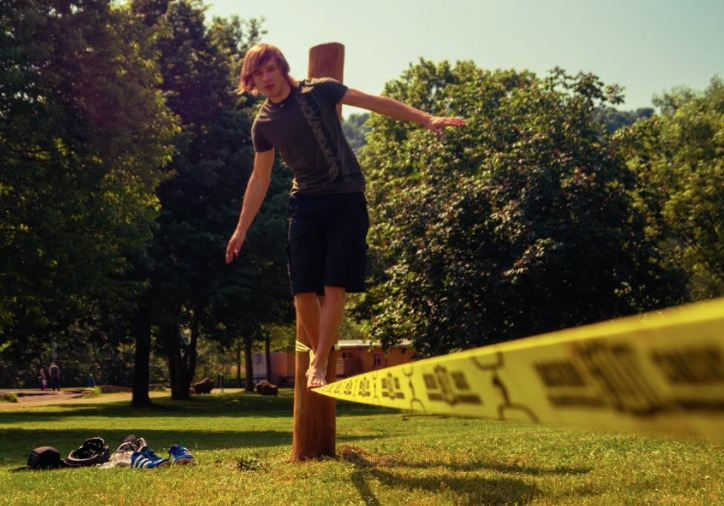
\includegraphics[width=0.7\linewidth]{Pictures/1_slackline}
		\caption{Person standing on a slackline and balancing out his sway}
		\label{fig:1_slackline}
	\end{minipage}
\end{figure}

These problems can be solved by an interactive slackline learning system.
The system presented in this thesis provides specific exercises as well as real-time support and feedback for beginners to learn slacklining.
%At the current stage of this thesis, no technology or application is known that provides 
Building a constructive predefined exercise routine with an appropriate difficulty level teaches the trainee how to stand and walk on a slackline from the ground up.
A detailed introduction with a preview of the exercise execution provides her with the appropriate knowledge for the ongoing exercise.
During the execution she gets audiovisual feedback about her execution in real-time with the help of several indicators.
Lastly, showing several performance parameters to summarize her learning progress of the exercise execution.


%The main skill acquisition technique for slacklining beginners is a personal trainer with intermediate expertise. Because of her experience she can provide useful tips, hints, and correct the slacker during the exercise execution. However the drawback is the dependency on the trainer. The slackline trainee has to know someone who can teach her slacklining. In reverse the dependency of the trainer to the trainee is also a drawback, since she has to look how good the exercises are executed. Further the trainee has to do several repetitive trials, to get familiar with her balancing actions and with the slackline. For this time range no trainer is needed, because she has to learn this movements by herself.

%In contrast to a personal human trainer the user is independent of any person. She is therefore 

%strengthens her general balance ability, introduces her to the slackline, and provide beginner exercises on it.

\begin{comment}
- no chance for beginners to learn it by herself correctly. Interactive assistance system would conquer these problems. No related work for this
-- In contrast to such a human personal trainer this thesis will elaborate an interactive slackline learning system with real-time feedback, called further SLS. 
-- Support slackline beginners with such a system

\textbf{-> Interaktive Systeme auf dem Markt}

-- Größtenteils genutzt für gaming

-- aber auch exergames großes potential

-- Home Training Assistent

\textbf{-> Einführung von exergames hiermit}

-- What are Exergames in general

-- Exergames positive impact on skill acquisition --> more exergames released in past decades?
---> Combining interactive technology in the context of learning or training skill for a sport activity within an application in a gaming approach is called

-- Several sports implemented

-- für Rehabilitation, krankengymnastik genutzt

-- Sportarten trainieren

-- Balance Sportarten/Activities

\textbf{-> Einführung von Slackline hiermit}

-- Kurze Slackline description

-- Slackline als sportart einführen

-- Normales lernprozedere erklären und assisstenzsystem erläutern / Mostly skill acquisition is done with a professional who already knows how to act on the line and where particular attention must be paid

-- Keine vergleichbare Interaktiven Anwendung für das Slacklinen / No comparable work relating to slacklining

-- In contrast to such a human personal trainer this thesis will elaborate an interactive slackline learning system with real-time feedback, called further SLS

-- Support slackline beginners with such a system
\end{comment}